%%%%%%%%%%%%%%%%%%%%%%%%%%%%%%%%%%%%%%%%%%%%%%%%%%%%%%%%%%%%%%%%%%%%%%%%%%%%%%%%%%%%
% Document data
%%%%%%%%%%%%%%%%%%%%%%%%%%%%%%%%%%%%%%%%%%%%%%%%%%%%%%%%%%%%%%%%%%%%%%%%%%%%%%%%%%%%
\documentclass[12pt]{report} %report allows for chapters
\renewcommand\thesection{\arabic{section}} % ignore the title number for sections
%%%%%%%%%%%%%%%%%%%%%%%%%%%%%%%%%%%%%%%%%%%%%%%%%%%%%%%%%%%%%%%%%%%%%%%%%%%%%%%%%%%%




%%%%%%%%%%%%%%%%%%%%%%%%%%%%%%%%%%%%%%%%%%%%%%%%%%%%%%%%%%%%%%%%%%%%%%%%%%%%%%%%%%%%
% Packages
%%%%%%%%%%%%%%%%%%%%%%%%%%%%%%%%%%%%%%%%%%%%%%%%%%%%%%%%%%%%%%%%%%%%%%%%%%%%%%%%%%%%
\usepackage{color, soul, xcolor} % Colored text and highlighting, respectively

%Tikz
\usepackage{tikz-cd} % For commutative diagrams
\usepackage{tikz-3dplot}
\RequirePackage{pgfplots}
\usetikzlibrary{shadows}
\usetikzlibrary{shapes}
\usetikzlibrary{decorations}
\usetikzlibrary{arrows,decorations.markings} 
\usetikzlibrary{quotes,angles}

\usepackage{mathtools}
\usepackage{answers}
\usepackage{setspace}
\usepackage{graphicx}
\usepackage{enumerate}
\usepackage{multicol}
\usepackage{mathrsfs}
\usepackage[margin=1in]{geometry} 
\usepackage{amsmath,amsthm,amssymb}
\usepackage{marvosym,wasysym} %fucking smileys
%%%%%%%%%%%%%%%%%%%%%%%%%%%%%%%%%%%%%%%%%%%%%%%%%%%%%%%%%%%%%%%%%%%%%%%%%%%%%%%%%%%%




%%%%%%%%%%%%%%%%%%%%%%%%%%%%%%%%%%%%%%%%%%%%%%%%%%%%%%%%%%%%%%%%%%%%%%%%%%%%%%%%%%%%
% Shortcuts
%%%%%%%%%%%%%%%%%%%%%%%%%%%%%%%%%%%%%%%%%%%%%%%%%%%%%%%%%%%%%%%%%%%%%%%%%%%%%%%%%%%%
% Number systems
\newcommand{\N}{\mathbb{N}}
\newcommand{\Z}{\mathbb{Z}}
\newcommand{\C}{\mathbb{C}}
\newcommand{\R}{\mathbb{R}}
\newcommand{\Q}{\mathbb{Q}}

% Operators/functions
\newcommand{\id}{\mathrm{Id}}
\DeclareMathOperator{\sech}{sech}
\DeclareMathOperator{\csch}{csch}
%%%%%%%%%%%%%%%%%%%%%%%%%%%%%%%%%%%%%%%%%%%%%%%%%%%%%%%%%%%%%%%%%%%%%%%%%%%%%%%%%%%%




%%%%%%%%%%%%%%%%%%%%%%%%%%%%%%%%%%%%%%%%%%%%%%%%%%%%%%%%%%%%%%%%%%%%%%%%%%%%%%%%%%%%
% Environments
%%%%%%%%%%%%%%%%%%%%%%%%%%%%%%%%%%%%%%%%%%%%%%%%%%%%%%%%%%%%%%%%%%%%%%%%%%%%%%%%%%%%
% Italic font
\newtheorem{theorem}{Theorem}[section]
\newtheorem{lemma}{Lemma}[section]
\newtheorem{corollary}{Corollary}[section]
\newtheorem{axiom}{Axiom}

% Plain font
\theoremstyle{definition}
\newtheorem{definition}{Definition}[section]
\newtheorem{example}{Example}[section]
\newtheorem{remark}{Remark}[section]
\newtheorem{solution}{Solution}
\newtheorem{problem}{Problem}[section]
\newtheorem{question}{Question}[section]
\newtheorem{answer}{Answer}[section]
\newtheorem{exercise}{Exercise}[section]
%%%%%%%%%%%%%%%%%%%%%%%%%%%%%%%%%%%%%%%%%%%%%%%%%%%%%%%%%%%%%%%%%%%%%%%%%%%%%%%%%%%%

\begin{document}


\begin{center}
   \textsc{\large MATH 255, Homework 3: \emph{Solutions}}\\
\end{center}
\vspace{.5cm}

\noindent\textbf{Relevant Sections:} 17.4, 17.5, 17.6, 18.4, 18.2, 18.6 \\

\noindent\textbf{Problem 1.} Consider the system of linear equations:
\begin{align*}
    3x+2y+0z&=5\\
    1x+1y+1z&=3\\
    0x+2y+2z&=4.
\end{align*}
\begin{enumerate}[(a)]
    \item Write the augmented matrix $M$ for this system of equations.
    \item Use row reduction to get the augmented matrix in row-echelon form.
    \item Determine the solution to the system of equations.
\end{enumerate}

\begin{solution}
\begin{enumerate}[(a)]
    \item We have
    \[
    M=\left[ \begin{array}{ccc|c}
        3 & 2 & 0 & 5\\
        1 & 1 & 1 & 3\\
        0 & 2 & 2 & 4
    \end{array}\right].
    \]
    \item We row reduce to the identity matrix on the left side of the bar.  So
    \[
    \textrm{Replace $R_2$ with $R_2-1/2 R_3$} ~\implies~     M=\left[ \begin{array}{ccc|c}
        3 & 2 & 0 & 5\\
        1 & 0 & 0 & 1\\
        0 & 2 & 2 & 4
    \end{array}\right]
    \]
    \[
    \textrm{Replace $R_1$ with $R_1-3 R_2$} ~\implies~     M=\left[ \begin{array}{ccc|c}
        0 & 2 & 0 & 2\\
        1 & 0 & 0 & 1\\
        0 & 0 & 2 & 2
    \end{array}\right]
    \]
    \[
    \textrm{Replace $R_3$ with $R_3- R_1$} ~\implies~     M=\left[ \begin{array}{ccc|c}
        0 & 2 & 0 & 2\\
        1 & 0 & 0 & 1\\
        0 & 0 & 2 & 2
    \end{array}\right]
    \]
    \[
    \textrm{Swap $R_1$ and $R_2$} ~\implies~     M=\left[ \begin{array}{ccc|c}
        1 & 0 & 0 & 1\\
        0 & 2 & 0 & 2\\
        0 & 0 & 2 & 2
    \end{array}\right]
    \]
    \[
    \textrm{Divide $R_2$ and $R_3$ by 2} ~\implies~     M=\left[ \begin{array}{ccc|c}
        1 & 0 & 0 & 1\\
        0 & 1 & 0 & 1\\
        0 & 0 & 1 & 1
    \end{array}\right]
    \]
    
    \item The above row reduction gives us the system
    \begin{align*}
        1x+0y+0z&=1\\
        0x+1y+0z&=1\\
        0x+0y+1z&=1
    \end{align*}
    which means that $x=y=z=1$.
\end{enumerate}
\end{solution}

\noindent\textbf{Problem 2.} Let
\[
A=\begin{bmatrix} 1 & 3 & 2 \\ 0 & 2 & 1\\ 2 & 1 & 2\\ \end{bmatrix} \quad \mathbf{b}= \begin{bmatrix} 1 \\ -3 \\ 13 \end{bmatrix}.
\]
\begin{enumerate}[(a)]
    \item Compute $\det(A)$ and determine whether the equation $A\mathbf{x}=\mathbf{b}$ has a solution.
    \item Create an augmented matrix $M$ for this system of equations.
    \item Determine the solution to the system of equations.
\end{enumerate}

\begin{solution}
\begin{enumerate}[(a)]
    \item To see whether this inhomogenous system has a unique solution, we take
    \[
    \det(A)=1.
    \]
    Since $\det(A)=1\neq 0$ we know that there exists a unique solution. (\emph{There are propositions for inhomogenous and homogeneous equations in the notes.  Be sure to take note of these.})
    
    \item We have
    \[
    M=\left[ \begin{array}{ccc|c}
        1 & 3 & 2 & 1\\
        0 & 2 & 1 & -3\\
        0 & 0 & 1/2 & 7/2
    \end{array}\right].
    \]
    
    \item We perform row reduction to get the identity on the left side of the bar in $M$.  I omit the steps here but you find that $x=2$, $y=-5$, and $z=7$ so that
    \[
    \mathbf{x}=\begin{bmatrix} 2 \\ -5 \\ 7 \end{bmatrix}.
    \]
\end{enumerate}
\end{solution}

\noindent\textbf{Problem 3.} Find the inverse matrix for each of the following:
\begin{enumerate}[(a)]
    \item \[
    A=\begin{bmatrix} 0 & 1 \\ -1 & 0 \end{bmatrix}.
    \]
    \item \[
    B=\begin{bmatrix} 1 & 1 & 0\\ 1 & 0 & 1 \\ 0 & 1 & 1 \end{bmatrix}.
    \]
\end{enumerate}

\begin{solution}
\begin{enumerate}[(a)]
    \item We create the augmented matrix
    \[
    M=\left[\begin{array}{cc|cc}
        0 & 1 & 1 & 0\\
        -1 & 0 & 0 & 1
    \end{array}\right].
    \]
    Then we row reduce the left hand side of the bar to the identity matrix.
    \[
    \textrm{Swap $R_1$ and $R_2$} ~\implies ~ \left[ \begin{array}{cc|cc}
        -1 & 0 & 0 & 1\\
        0 & 1 & 1 & 0
    \end{array}\right]
    \]
    \[
    \textrm{Multiply $R_1$ by $-1$} ~\implies ~ \left[ \begin{array}{cc|cc}
        1 & 0 & 0 & -1\\
        0 & 1 & 1 & 0
    \end{array}\right].
    \]
    So we have
    \[
    A^{-1}=\begin{bmatrix} 0 & -1\\ 1 & 0\end{bmatrix}.
    \]
    We can verify this by
    \[
    A^{-1}A = \begin{bmatrix} 0 & -1 \\ 1 & 0 \end{bmatrix} \begin{bmatrix} 0 & 1\\ -1 & 0 \end{bmatrix} = \begin{bmatrix} 1 & 0 \\ 0 & 1 \end{bmatrix}.
    \]
    
    \item We repeat this process again.  First we make
    \[
    M= \left[ \begin{array}{ccc|ccc}
        1 & 1 & 0 & 1 & 0 & 0\\
        1 & 0 & 1 & 0 & 1 & 0\\
        0 & 1 & 1 & 0 & 0 & 1
    \end{array}
    \right].
    \]
    We then row reduce the left side of the bar to the identity matrix.  I omit the work here, but in the end you have
    \[
    \left[ \begin{array}{ccc|ccc|}
        1 & 0 & 0 & 1/2 & 1/2 & -1/2\\
        0 & 1 & 0 & 1/2 & -1/2 & 1/2\\
        0 & 0 & 1 & -1/2 & 1/2 & 1/2
    \end{array}\right].
    \]
    So we have
    \[
    B^{-1}=\begin{bmatrix} 1/2 & 1/2 & -1/2 \\ 1/2 & -1/2 & 1/2 \\ -1/2 & 1/2 & 1/2 \end{bmatrix}.
    \]
    You can perform the same check as we did for the previous part.
\end{enumerate}
\end{solution}

\noindent\textbf{Problem 4.} Construct transformation matrices that represent the following rotations about the $z$-axis:
\begin{enumerate}[(a)]
    \item Counterclockwise through $45^\circ = \frac{\pi}{4}$.
    \item Counterclockwise through $90^\circ = \frac{\pi}{2}$.
    \item Clockwise through $90^\circ = \frac{\pi}{2}$.
\end{enumerate}
(\emph{Hint: This necessary matrix is given to you in the notes and in the book, chapter 18).}

\begin{solution}
The book provides us the matrix
\[
R= \begin{bmatrix} \cos \theta & - \sin \theta \\ \sin \theta & \cos \theta \end{bmatrix}
\]
which rotates a vector in the plane by an angle $\theta$ in the counterclockwise direction.  However, it is worth looking to see how this is derived (though I did not want you to derive this yourself).

Recall from Homework 2 Problem 4 that we can understand a linear transformation entirely by how it transforms the basis vectors.  In this case, we want
\[
R\left( \begin{bmatrix} 1 \\ 0 \end{bmatrix} \right) \qquad R\left(\begin{bmatrix} 0 \\ 1\end{bmatrix} \right)
\]
to each be rotated by an angle $\theta$.  So we draw the following
\begin{figure}[h]
    \centering
    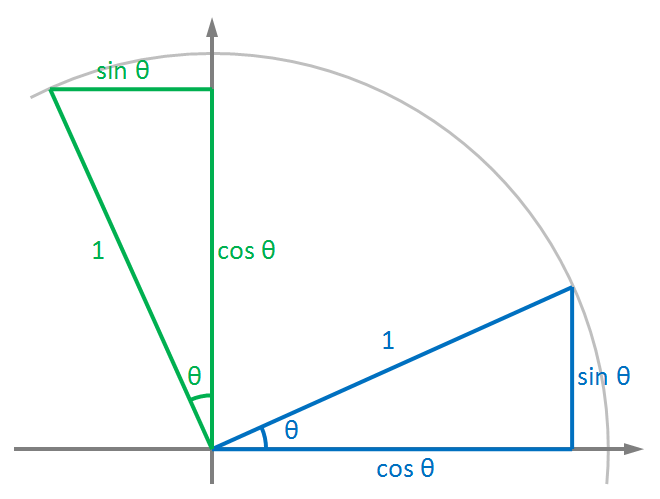
\includegraphics[width=.5\textwidth]{Images/rotation.png}
\end{figure}
Here we notice that
\[
R\left( \begin{bmatrix} 1 \\ 0 \end{bmatrix}\right) = \begin{bmatrix} \cos \theta \\ \sin \theta \end{bmatrix}
\]
and
\[
R\left( \begin{bmatrix} 0 \\ 1 \end{bmatrix}\right) = \begin{bmatrix} -\sin \theta \\ \cos \theta \end{bmatrix}.
\]
This leads us exactly to 
\[
R=\begin{bmatrix} \cos \theta & -\sin \theta \\ \sin \theta & \cos \theta \end{bmatrix}.
\]

\begin{enumerate}[(a)]
    \item We plug in $\theta_a = \pi/4$ and find
    \[
    R_a = \begin{bmatrix} \frac{1}{\sqrt{2}} & -\frac{1}{\sqrt{2}}\\ \frac{1}{\sqrt{2}} & \frac{1}{\sqrt{2}}\end{bmatrix}.
    \]
    
    \item We plug in $\theta_b = \pi/2$ and find
    \[
    R_b = \begin{bmatrix} 0 & -1 \\ 1 & 0\end{bmatrix}.
    \]
    
    \item We plug in $\theta_c = -\pi/2$ since a negative angle will rotate clockwise.  Then we get
    \[
    R_c = \begin{bmatrix} 0 & 1 \\ -1 & 0 \end{bmatrix}.
    \]
\end{enumerate}

\end{solution}

\noindent\textbf{Problem 5.} Find the eigenvalues and eigenvectors for the following matrices.
\begin{enumerate}[(a)]
    \item \[
    A= \begin{bmatrix} 5/2 & 1/2 \\ 1/2 & 5/2 \end{bmatrix}.
    \]
    \item \[
    B= \begin{bmatrix} -1/2 & 1/2 & -1/2 \\ -1/2 & 1/2 & 1/2 \\ -1 & 1 & 0\end{bmatrix}.
    \]
\end{enumerate}

\begin{solution}
\begin{enumerate}[(a)]
    \item First, we take
    \[
    \det(A-\lambda I)=\left| \begin{array}{cc}
        5/2-\lambda & 1/2 \\ 1/2 & 5/2-\lambda`
    \end{array}\right| = (5/2-\lambda)^2-1/4.
    \]
    We set this equal to zero and simplify to find
    \begin{align*}
    \lambda^2+5\lambda+6&=0\\
    (\lambda-2)(\lambda-3)&=0
    \end{align*}
    meaning that we have $\lambda_1=2$ and $\lambda_2=3$. Then we find each eigenvector. 
    
    \noindent\underline{For $\lambda_1=2$:}
    
    We solve 
    \[
    (A-2I)\mathbf{v}_1=\mathbf{0}.
    \]
    Writing this out as an augmented matrix, we get
    \[
    M=\left[ \begin{array}{cc|c}
        1/2 & 1/2 & 0\\
        1/2 & 1/2 & 0
    \end{array}\right]
    \]
    Row reducing as much as we can gives us
    \[
    \left[ \begin{array}{cc|c}
        1 & 1 & 0\\
        0 & 0 & 0
    \end{array}\right]
    \]
    and the system of equations
    \begin{align*}
        1x + 1y &=0\\
        0x+0y&=0.
    \end{align*}
    The second equation means that $y$ is a free variable.  I'll choose $y=1$.  Then we get that $x=-y$ from the first equation.  So we have that
    \[
    \mathbf{v}_1=\begin{bmatrix} 1 \\ -1 \end{bmatrix}.
    \]
    Of course, you can choose any nonzero value for $y$.
    
    \noindent\underline{For $\lambda_2=3$:}
    
    We solve 
    \[
    (A-3I)\mathbf{v}_2&=\mathbf{0}.
    \]
    Writing this out as an augmented matrix, we get
    \[
    M=\left[ \begin{array}{cc|c}
        -1/2 & 1/2 & 0\\
        1/2 & -1/2 & 0
    \end{array}\right]
    \]
    Row reducing as much as we can gives us
    \[
    \left[ \begin{array}{cc|c}
        -1 & 1 & 0\\
        0 & 0 & 0
    \end{array}\right]
    \]
    and the system of equations
    \begin{align*}
        -1x + 1y &=0\\
        0x+0y&=0.
    \end{align*}
    The second equation means that $y$ is a free variable.  I'll choose $y=1$.  Then we get that $x=y$ from the first equation.  So we have that
    \[
    \mathbf{v}_2=\begin{bmatrix} 1 \\ 1 \end{bmatrix}.
    \]
    
    Fun fact: If we take the eigenvectors and place them in a matrix
    \[
    P=\begin{bmatrix} \mathbf{v}_1 & \mathbf{v}_2 \end{bmatrix} = \begin{bmatrix} 1 & 1 \\ -1 & 1\end{bmatrix}.
    \]
    Then we can write
    \[
    A=PDP^{-1}
    \]
    where
    \[
    D=\begin{bmatrix} 2 & 0\\ 0 & 3 \end{bmatrix}
    \]
    is a diagonal matrix containing the eigenvalues of $A$ along the diagonal.  This is where the name \emph{diagonalization} comes from.  This process can be generalized and it yields what is called the \emph{singular value decomposition} or SVD.  SVD is widely used in data analysis and is an extremely important result of linear algebra!
    
    \item We repeat the usual process here.  First
    \begin{align*}
        \det(B-\lambda I)&=0\\
        \implies \lambda-\lambda^3&=0\\
        \implies \lambda(\lambda-1)(\lambda+1)&=0.
    \end{align*}
    So the eigenvalues are 
    \[
    \lambda_1 = 0 \qquad \lambda_2 = 1 \qquad \lambda_3=-1.
    \]
    I omit the work here, but the corresponding eigenvectors are
    \[
    \mathbf{v}_1= \begin{bmatrix} 1\\ 1\\ 0 \end{bmatrix} \qquad \mathbf{v}_1=\begin{bmatrix} 0 \\ 1 \\ 1 \end{bmatrix} \qquad \mathbf{v}_3=\begin{bmatrix} 1 \\ 0 \\ 1\end{bmatrix}.
    \]
    
\end{enumerate}
\end{solution}






\end{document}  